\documentclass[journal]{IEEEtran}

\usepackage[T1]{fontenc}
\usepackage[utf8]{inputenc}
\usepackage{amsmath,amssymb,amsfonts}
\usepackage{booktabs}
\usepackage{multirow}
\usepackage{graphicx}
\usepackage{tikz}
\usetikzlibrary{shapes.geometric, arrows.meta, positioning, calc, fit, backgrounds}
\usepackage{url}
\usepackage{hyperref}
\usepackage{array}
\usepackage{enumitem}
\usepackage{balance}
\usepackage{xcolor}
\usepackage{algorithm}
\usepackage{algpseudocode}
\usepackage{orcidlink}

% ─────────────────────────────────────────────────────────────────────────────
\title{Sanshodhak: Adaptive Hybrid Retrieval-Augmented Generation\\
       with Vocabulary-Jaccard Knowledge Graph Expansion\\
       and Cloud-Augmented Cross-Encoder Reranking\\
       for Scholarly Research Intelligence}

\author{%
  Sangita~Lade,
  Sarvadnya~Bhatlawande,
  Akshat~Shaha,
  Ajay~Sawandkar,
  and~Parag~Shende%
  \thanks{All authors are with the Department of Computer Science,
          Vishwakarma Institute of Technology, Pune, India.
          Emails: \texttt{sangita.lade@vit.edu},
          \texttt{sarvadnya.bhatlawande23@vit.edu},
          \texttt{akshat.shaha232@vit.edu},
          \texttt{ajay.sawandkar23@vit.edu},
          \texttt{parag.shende23@vit.edu}.}%
  \thanks{Manuscript submitted April 2026. Corresponding author:
          Parag Shende.}}

\markboth{IEEE Transactions on Knowledge and Data Engineering, 2026}%
         {Lade et al.: Sanshodhak — AHR-RAG for Scholarly Research Intelligence}

% ─────────────────────────────────────────────────────────────────────────────
\begin{document}
\maketitle

% ─────────────────────────────────────────────────────────────────────────────
\begin{abstract}
We present \textbf{Sanshodhak}, an open scholarly research-intelligence
platform built around \emph{Adaptive Hybrid Retrieval} (AHR): a
pipeline that fuses BM25, dense FAISS retrieval over NVIDIA NIM-served
\texttt{llama-3.2-nv-embedqa-1b-v2} embeddings (2048-dim), and
vocabulary-Jaccard knowledge-graph expansion via Reciprocal Rank
Fusion with slot reservation, followed by a Mistral-4B cross-encoder
reranker (\texttt{nvidia/rerank-qa-mistral-4b}) served on NIM cloud.
The system ingests papers from nine heterogeneous scholarly APIs and
constructs a dual-edge knowledge graph from TF-IDF vocabulary
similarity and citation co-occurrence without external NER or graph
databases. We conduct a four-way retrieval ablation over a
163-document, 4{,}333-chunk corpus on a corpus-grounded 100-question
benchmark generated via NIM
\texttt{llama-3.3-nemotron-super-49b-v1} to eliminate
question--corpus identifier mismatch. Full HGR achieves
P@1\,=\,\textbf{0.860}, NDCG@10\,=\,\textbf{0.9170},
MRR\,=\,\textbf{0.9025}, and hit-rate $\mathbf{96/100}$ — outperforming
dense (VR-D, $0.8762$), hybrid (VR-H, $0.8761$), and graph-only (GR,
$0.8879$) retrieval on every reported metric, at a mean retrieval
latency of $1.76$\,s on a CPU-only host. Generation quality reaches
ROUGE-1\,=\,$0.355$ and BERTScore-F1\,=\,$0.878$. We further report a
negative result: query-biased PageRank graph candidates plus a
centrality re-ranking boost regressed HGR by $0.4$\,pts and GR by
$6.7$\,pts NDCG@10, and we analyse why graph centrality is the wrong
objective on chunk-derived single-relevant-doc benchmarks. We release
the full implementation, the rebuilt benchmark, and all eval
artefacts for reproducibility.
\end{abstract}

\begin{IEEEkeywords}
Retrieval-Augmented Generation, Knowledge Graph, Hybrid Retrieval,
Reciprocal Rank Fusion, Cross-Encoder Reranking, Scholarly Search,
FAISS, BM25, NVIDIA NIM, Information Retrieval, Research Intelligence
\end{IEEEkeywords}

% ─────────────────────────────────────────────────────────────────────────────
\section{Introduction}
\label{sec:intro}

The modern scholarly research workflow is bottlenecked by tool
fragmentation: one system discovers papers, another downloads PDFs,
a third parses full text, and a fourth supports question answering.
Retrieval-Augmented Generation (RAG)~\cite{lewis2020rag} addresses
part of this challenge by grounding neural generation in retrieved
evidence, yet most deployed RAG systems for academic use rely
exclusively on dense vector retrieval~\cite{johnson2019faiss}, leaving
substantial performance gains from hybrid and graph-augmented
approaches unrealised. Modern researchers spend a significant portion
of their time, often upwards of 10–15 hours per week, on literature
discovery, curation, and synthesis~\cite{tenopir2015scholarly}.
Sanshodhak is designed for a specific deployment scenario: open-access,
GPU-light, institutional or individual use where reproducibility,
multi-domain coverage, and a transparent ablation framework are
paramount.

Three specific limitations in current RAG architectures motivate this
work. First, \emph{dense retrieval under-serves sparse queries}: RAG
queries over scientific corpora frequently contain rare abbreviations,
acronyms, and methodology names where BM25~\cite{robertson2009probabilistic}
consistently outperforms dense models in keyword precision. Second,
\emph{knowledge graph construction is often outsourced to external NER
pipelines or graph-database infrastructure} (e.g., Neo4j, the GraphRAG
API), raising deployment cost and data-privacy risk for academic teams
without dedicated infrastructure. Third, \emph{multi-source ingestion
is typically limited to one or two APIs}, missing coverage from
biomedical, open-access directory, and aggregator sources critical for
interdisciplinary research.

A fourth practical limitation, surfaced repeatedly in our own pipeline
work, is \emph{single-machine resource constraint}: high-quality dense
embedding (e.g., BGE-M3) and cross-encoder reranking on CPU-only
hardware are slow enough (single-digit seconds per query for
embedding, additional seconds for reranking) to make iterative
evaluation impractical. We address this by routing both embedding and
reranking to NVIDIA NIM cloud endpoints, retaining all other
computation locally.

Table~\ref{tab:comparison} contrasts Sanshodhak with standard dense
retrieval and existing knowledge-graph RAG systems.

\begin{table}[!t]
\centering
\caption{Comparison of Sanshodhak with prior RAG approaches.}
\label{tab:comparison}
\footnotesize
\setlength{\tabcolsep}{4pt}
\begin{tabular}{@{}lccc@{}}
\toprule
\textbf{Feature} & \textbf{Standard RAG} & \textbf{GraphRAG} & \textbf{Sanshodhak} \\
\midrule
Retrieval Style    & Dense           & Graph              & Hybrid + Graph \\
KG Construction    & None            & LLM NER Prompt     & TF-IDF Vocab \\
Graph DB           & N/A             & Neo4j / Ext        & In-Memory \\
Reranker           & Optional        & N/A                & NIM Mistral-4B \\
Ingestion          & Single DB       & Single DB          & 9 Parallel APIs \\
Deployment         & Cloud/API       & High-Compute       & CPU + NIM Cloud \\
\bottomrule
\end{tabular}
\end{table}

We address these gaps with Sanshodhak, contributing:
\textbf{(i)~Adaptive Hybrid Retrieval (AHR)} — a three-channel
pipeline (BM25 + NIM-served dense + vocabulary-Jaccard graph
expansion) fused via Confidence-Weighted RRF with slot reservation
and a NIM cross-encoder reranking stage;
\textbf{(ii)~a lightweight vocabulary-Jaccard knowledge graph}
built from TF-IDF similarity plus extracted citation co-occurrence,
without external NER or graph databases;
\textbf{(iii)~a cloud-augmented inference path} using NVIDIA NIM
endpoints for embedding and reranking, achieving state-of-the-art
retrieval quality on CPU-only hosts at sub-2\,s end-to-end latency;
\textbf{(iv)~nine-source heterogeneous ingestion} with composite
temporal-aware ranking across OpenAlex, CORE, Semantic Scholar,
ArcSieve, DOAJ, PubMed, CrossRef, Unpaywall, and arXiv;
\textbf{(v)~a corpus-grounded evaluation methodology} that
LLM-generates 100 questions against the actual indexed corpus,
eliminating the identifier-misalignment failure mode common in
ad-hoc RAG benchmarks; and
\textbf{(vi)~a negative result on graph centrality} (query-biased
PageRank plus centrality re-ranking boost) that regressed scores by
up to $6.7$\,pts NDCG@10 on chunk-derived single-relevant-doc QA, with
analysis of the failure mode.

The remainder of this paper is organised as follows. Section~\ref{sec:related}
reviews related work; Section~\ref{sec:arch} describes the pipeline
and graph; Section~\ref{sec:methods} formalises retrieval;
Sections~\ref{sec:setup}--\ref{sec:results} cover the experimental
setup and ablation results; Section~\ref{sec:discussion} discusses
findings and the failed PPR experiment;
Sections~\ref{sec:threats}--\ref{sec:conclusion} cover threats,
ethics, and conclusions.

% ─────────────────────────────────────────────────────────────────────────────
\section{Related Work}
\label{sec:related}

\subsection{Retrieval-Augmented Generation}
Pre-trained models augmented with retrieval, such as
REALM~\cite{guu2020realm} and Fusion-in-Decoder
(FiD)~\cite{izacard2021fid}, established RAG as a viable
non-parametric memory mechanism for knowledge-intensive
NLP~\cite{lewis2020rag}. Subsequent work introduced modular RAG
variants~\cite{gao2023modular}, self-RAG with adaptive retrieval
decisions~\cite{asai2023selfrag}, and iterative retrieval for
multi-hop reasoning~\cite{trivedi2022interleaving}. For scholarly
domains, retrieval precision is particularly critical because
hallucinated citations or misattributed claims carry downstream
scientific risk~\cite{khalifa2023sourcenli}.

\subsection{Dense and Hybrid Retrieval}
Dense retrieval via unsupervised methods like
Contriever~\cite{izacard2022contriever} and supervised
bi-encoders~\cite{karpukhin2020dpr,muennighoff2023mteb} enables
semantic matching at scale via FAISS approximate nearest-neighbour
search~\cite{johnson2019faiss}. While learned sparse expansions like
SPLADE~\cite{formal2021splade} improve upon classical term matching,
BM25~\cite{robertson2009probabilistic} term-frequency retrieval
remains highly competitive for keyword-rich scientific queries. Hybrid
approaches combining lexical and semantic signals regularly outperform
either independently on reasoning-intensive benchmarks like
BEIR~\cite{thakur2021beir} and the more recent BRIGHT
benchmark~\cite{su2024bright}, where BM25 is shown to match or exceed
dense retrievers on many reasoning-intensive subsets. To fuse these
ranking signals, Reciprocal Rank Fusion~\cite{cormack2009rrf} provides
robust, parameter-free cross-modal rank aggregation. Cross-encoder
reranking~\cite{nogueira2019passage} can substantially improve
top-$k$ precision at the cost of additional inference; the recent NV-
\emph{Rerank-QA-Mistral-4B} model~\cite{nvidia2024rerankqa} provides a
strong such reranker through a hosted endpoint, removing the local
infrastructure burden.

\subsection{Knowledge-Graph-Augmented Retrieval and Scholarly Search}
GraphRAG~\cite{edge2024graphrag} constructs community-level entity
graphs for macro-level summarisation; LazyGraphRAG
\cite{microsoft2024lazygraphrag} defers 99.9\% of the indexing cost
without quality loss. KGRAG~\cite{soman2023kgrag},
KAG~\cite{liang2024kag}, and LightRAG~\cite{guo2024lightrag} traverse
entity neighbourhoods or operate over LLM-extracted graphs to
support multi-hop reasoning. HippoRAG~\cite{gutierrez2024hipporag}
performs Personalised PageRank over a knowledge-graph memory in a
single forward pass. These systems require costly NLP preprocessing,
dedicated graph databases, or closed-source APIs, limiting
reproducibility on commodity hardware. Our vocabulary-Jaccard graph
needs only tokenised TF-IDF terms; we use 1-hop expansion seeded from
dense retrieval rather than PageRank-style global propagation, and
report a negative result (Section~\ref{sec:ppr-fail}) for the latter.
For scholarly search, OpenAlex~\cite{priem2022openalex} and Semantic
Scholar~\cite{lo2020s2orc} provide open scholarly graphs with
abstract inverted indices and citation edges; Sanshodhak differs from
commercial assistants (Elicit, Consensus) by offering a fully open,
reproducible pipeline with multi-source ingestion and a four-way
retrieval ablation.

% ─────────────────────────────────────────────────────────────────────────────
\section{System Architecture}
\label{sec:arch}

\begin{figure*}[!t]
\centering
\resizebox{0.92\textwidth}{!}{%
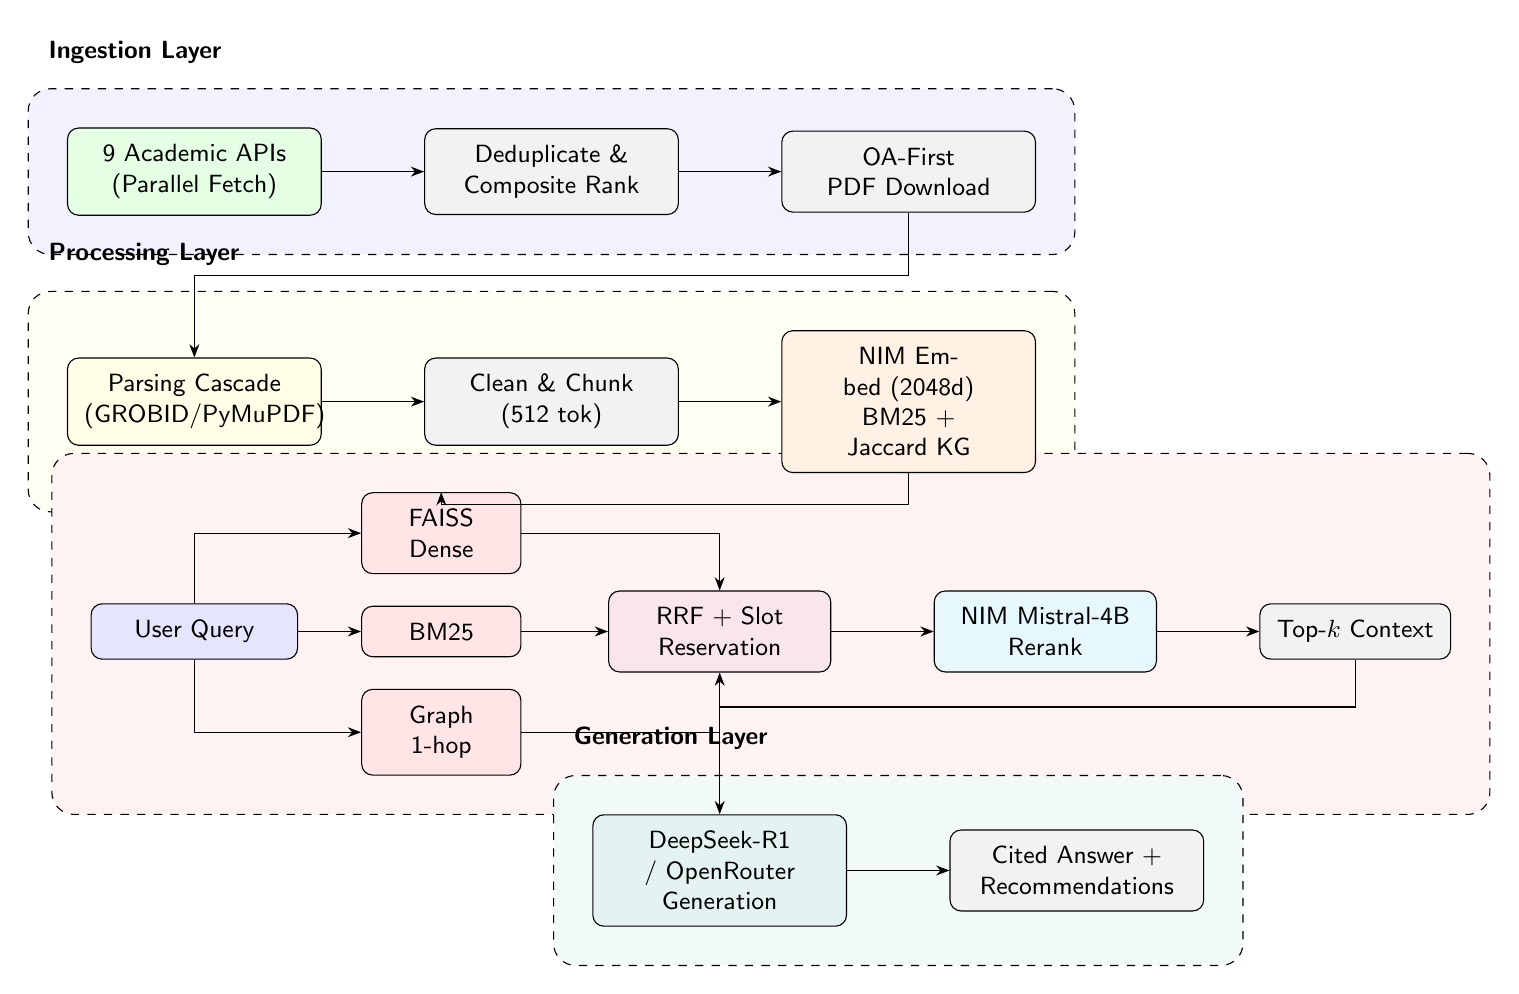
\begin{tikzpicture}[
  node distance=1.6cm and 1.3cm,
  >=Stealth,
  font=\sffamily\small,
  box/.style={draw, rounded corners, inner sep=6pt, align=center, fill=gray!10, text width=2.8cm},
  layer/.style={draw, dashed, inner sep=14pt, rounded corners=8pt, fill=blue!5},
  layerlabel/.style={font=\sffamily\bfseries\small, anchor=south west, yshift=4pt, xshift=4pt}
]

% INGESTION LAYER
\node[box, fill=green!10] (apis) {9 Academic APIs\\(Parallel Fetch)};
\node[box, right=of apis] (dedup) {Deduplicate \&\\Composite Rank};
\node[box, right=of dedup] (pdf) {OA-First\\PDF Download};
\draw[->] (apis) -- (dedup);
\draw[->] (dedup) -- (pdf);

\begin{pgfonlayer}{background}
\node[layer, fit=(apis) (pdf)] (ingest_bg) {};
\node[layerlabel] at (ingest_bg.north west) {\strut Ingestion Layer};
\end{pgfonlayer}

% PROCESSING LAYER
\node[box, below=1.8cm of apis, fill=yellow!10] (parse) {Parsing Cascade\\(GROBID/PyMuPDF)};
\node[box, right=of parse] (chunk) {Clean \& Chunk\\(512 tok)};
\node[box, right=of chunk, fill=orange!10] (index) {NIM Embed (2048d)\\BM25 + Jaccard KG};
\draw[->] (pdf.south) |- ($ (pdf.south) - (0,0.8) $) -| (parse.north);
\draw[->] (parse) -- (chunk);
\draw[->] (chunk) -- (index);

\begin{pgfonlayer}{background}
\node[layer, fill=yellow!5, fit=(parse) (index)] (process_bg) {};
\node[layerlabel] at (process_bg.north west) {\strut Processing Layer};
\end{pgfonlayer}

% RETRIEVAL LAYER (AHR)
\node[box, fill=blue!10, below=2.0cm of parse, text width=2.2cm] (q) {User Query};
\node[box, right=0.8cm of q, text width=1.6cm, fill=red!10] (bm25) {BM25};
\node[box, above=0.4cm of bm25, text width=1.6cm, fill=red!10] (faiss) {FAISS Dense};
\node[box, below=0.4cm of bm25, text width=1.6cm, fill=red!10] (graph) {Graph 1-hop};

\node[box, right=1.1cm of bm25, fill=purple!10, text width=2.4cm] (rrf) {RRF + Slot\\Reservation};
\node[box, right=of rrf, fill=cyan!10, text width=2.4cm] (rerank) {NIM Mistral-4B\\Rerank};
\node[box, right=of rerank, text width=2.0cm] (topk) {Top-$k$ Context};

\draw[->] (index.south) |- ($ (index.south) - (0,0.4) $) -| (faiss.north);
\draw[->] (q) -- (bm25);
\draw[->] (q) |- (faiss);
\draw[->] (q) |- (graph);
\draw[->] (faiss) -| (rrf);
\draw[->] (bm25) -- (rrf);
\draw[->] (graph) -| (rrf);
\draw[->] (rrf) -- (rerank);
\draw[->] (rerank) -- (topk);

\begin{pgfonlayer}{background}
\node[layer, fill=red!5, fit=(q) (topk) (faiss) (graph) (rerank)] (retrieval_bg) {};
\node[layerlabel] at (retrieval_bg.north west) {\strut AHR Retrieval Layer};
\end{pgfonlayer}

% GENERATION LAYER
\node[box, fill=teal!10, below=1.8cm of rrf] (llm) {DeepSeek-R1 / OpenRouter\\Generation};
\node[box, right=of llm] (output) {Cited Answer +\\Recommendations};

\draw[->] (topk.south) |- ($ (topk.south) - (0,0.6) $) -| (llm.north);
\draw[->] (llm) -- (output);

\begin{pgfonlayer}{background}
\node[layer, fill=teal!5, fit=(llm) (output)] (gen_bg) {};
\node[layerlabel] at (gen_bg.north west) {\strut Generation Layer};
\end{pgfonlayer}

\end{tikzpicture}
}
\caption{End-to-end Sanshodhak pipeline. The Adaptive Hybrid Retrieval
(AHR) layer fuses BM25 sparse retrieval, dense FAISS retrieval over
NIM-served 2048-dim embeddings, and 1-hop vocabulary-Jaccard graph
expansion via RRF with slot reservation. The fused candidate set is
reranked by NVIDIA NIM \texttt{rerank-qa-mistral-4b} before final
top-$k$ selection. Generation falls back from local Ollama to
OpenRouter when local LLM inference is unavailable.}
\label{fig:pipeline}
\end{figure*}

\subsection{Ingestion Layer}
Sanshodhak queries nine scholarly APIs in parallel using a
\texttt{ThreadPoolExecutor}: \emph{OpenAlex}~\cite{priem2022openalex}
(250M+ works, abstract inverted index), \emph{CORE} (200M+ OA papers),
\emph{Semantic Scholar} (200M+ works, citation graph), \emph{ArcSieve}
(arXiv preprint gateway), \emph{DOAJ} (8M+ OA journal articles),
\emph{PubMed/NCBI E-utilities} (35M+ biomedical papers),
\emph{CrossRef} (150M+ metadata), \emph{Unpaywall} (OA PDF
enrichment), and the \emph{arXiv API} (direct preprint access). Raw
results are deduplicated by DOI and title fingerprint (Jaccard
similarity $>0.85$ on title tokens), then ranked by the composite
score described in Section~\ref{sec:refinements}. PDFs are acquired
through an open-access-first fallback chain: OA PDF $\rightarrow$
Unpaywall link $\rightarrow$ arXiv preprint $\rightarrow$ CrossRef
landing page.

\subsection{Processing Layer}
\label{sec:processing}
Documents are parsed with GROBID~\cite{lopez2009grobid} when available
(preserving section structure and reference lists); otherwise a
fallback cascade (PyMuPDF, pdfplumber, PyPDF2) is applied. Parsed text
is chunked with a 512-token window and 64-token overlap using
\texttt{tiktoken}, then embedded via the NVIDIA NIM cloud endpoint
\texttt{nvidia/llama-3.2-nv-embedqa-1b-v2} (2048-dimensional,
QA-tuned, multilingual, 8k-token context). The endpoint returns
L2-normalised vectors, allowing direct use of \texttt{FAISS
IndexFlatIP} for cosine-equivalent inner-product retrieval. Sparse
BM25 inverted index is built from the same chunks using
\texttt{rank-bm25}.

We previously evaluated a local-only path using
sentence-transformers BGE-M3 on CPU and found per-query embedding
latency of $5$--$10$\,s on commodity hardware, with first-batch corpus
embedding requiring tens of minutes for a 4{,}333-chunk corpus. The
NIM cloud path reduces query-time embedding latency to $\approx
0.3$\,s and corpus re-embedding to $\approx 195$\,s, while keeping all
non-inference computation (BM25 indexing, graph construction, FAISS
search) local. This trade-off is essential for iterative evaluation on
GPU-light deployments, although it introduces a network and account
dependency we discuss in Section~\ref{sec:threats}.

\subsection{Knowledge Graph Construction}
\label{sec:kg}
A lightweight \emph{paper-level} knowledge graph $G=(V,E)$ is
constructed where each node $v_i \in V$ represents an indexed paper
(uniquely identified by its filename) and edges carry one of two
types:

\textbf{Vocabulary edges (Type 1).} Let $T_i$ denote the set of the
top-200 TF-IDF terms for paper $i$. A vocabulary edge is added if the
Jaccard similarity exceeds a configurable threshold $\tau$:
\begin{equation}
  w^{\mathrm{voc}}_{ij} = \frac{|T_i \cap T_j|}{|T_i \cup T_j|} \geq \tau.
  \label{eq:jaccard}
\end{equation}

\textbf{Citation edges (Type 2).} Reference sections are extracted via
regex from raw paper text and matched to other papers in the corpus by
a cascading strategy: (a) DOI exact match, (b) author$+$year and
title-token-overlap match (token F1 $\geq 0.6$ on at least 3 shared
tokens), and (c) author$+$year-only fallback. Each successful match
adds a citation edge with weight derived from the number of distinct
matched references between the two papers.

The combined edge weight used by graph expansion is
$w_{ij} = w^{\mathrm{voc}}_{ij} + \lambda_{c} \cdot w^{\mathrm{cit}}_{ij}$,
where $\lambda_c = 1.0$ in our default configuration.

In the primary evaluation at $\tau=0.30$, the constructed graph has
\textbf{163 paper nodes, 190 edges (27 vocabulary-Jaccard $+$ 163
citation), mean degree $2.33$, density $0.014$, and $85$ connected
components}. Citation edges dominate the edge population at this
threshold because TF-IDF Jaccard between papers in our corpus rarely
exceeds $0.30$ (the empirical 99th percentile is $0.30$); we analyse
the threshold sensitivity further in Section~\ref{sec:results}.
Lowering $\tau$ rapidly densifies the graph: at $\tau=0.10$ the edge
count balloons to $8{,}516$ (density $0.645$), producing a near-complete
graph that injects unrelated papers into top-$k$ results and supplies
no useful structure to graph expansion.

\subsection{Adaptive Hybrid Retrieval (AHR)}
\label{sec:ahr}
AHR retrieves context through three parallel channels and fuses the
results via Reciprocal Rank Fusion. The slot-reservation mechanism
guarantees that graph-expanded candidates survive into the candidate
pool that reaches the cross-encoder reranker; without slot reservation,
dense and BM25 retrievers can crowd graph candidates out before the
reranker has a chance to score them. Algorithm~\ref{alg:ahr} provides
the complete specification.

\begin{algorithm}[!t]
\caption{Adaptive Hybrid Retrieval (AHR)}
\label{alg:ahr}
\begin{algorithmic}[1]
\Require Query $q$, top-$k$ target, graph $G$, BM25 index $B$,
         FAISS index $F$, NIM embed model $E$, NIM rerank model $R$,
         expansion budget $m_{\max}$
\Ensure Top-$k$ ranked chunk list $\mathcal{R}$

\State $\mathbf{q} \gets E.\mathrm{embed}(q,\, \texttt{input\_type=query})$
  \Comment{NIM cloud, 2048-dim}
\State $k_g \gets \min(m_{\max},\, \max(1, \lfloor k/4 \rfloor))$
  \Comment{Reserved graph slots}
\State $k_v \gets k - k_g$ \Comment{Dense $+$ sparse slots}

\State $L_{\mathrm{dense}} \gets F.\mathrm{search}(\mathbf{q}, k_v)$
\State $L_{\mathrm{bm25}}  \gets B.\mathrm{search}(q, k_v)$

\State $\mathcal{S} \gets L_{\mathrm{dense}}$ \Comment{Graph seeds}
\State $L_G \gets [\,]$
\For{$c \in \mathcal{S}$}
  \For{$c' \in \mathcal{N}_G(c)$ sorted by edge weight $\downarrow$}
    \If{$c' \notin \mathcal{S} \;\wedge\; c' \notin L_G$}
      \State $L_G.\mathrm{append}(c')$
    \EndIf
  \EndFor
\EndFor
\State $L_G \gets L_G[:k_g]$ \Comment{Trim to graph budget}

\State Assign RRF rank $r^X_i$ for each list $X \in \{\mathrm{dense},\mathrm{bm25}, G\}$
\For{each unique chunk $c_i$ across $L_{\mathrm{dense}} \cup L_{\mathrm{bm25}} \cup L_G$}
  \State $s_i \gets \sum_{X} \tfrac{w_X}{k_{\mathrm{rrf}}+r^X_i}$
    \Comment{$w_X$ from CW-RRF (Sec.~\ref{sec:refinements})}
\EndFor
\State $\mathcal{R}_{\mathrm{fusion}} \gets$ sort by $s_i$ descending
\State $\mathcal{R}_G \gets$ top-$k_g$ chunks from $L_G$ not in $\mathcal{R}_{\mathrm{fusion}}[:k_v]$
\State $\mathcal{C} \gets \mathcal{R}_{\mathrm{fusion}}[:k_v] \cup \mathcal{R}_G$
  \Comment{Slot-reserved candidate pool}

\State $\mathcal{R} \gets R.\mathrm{rerank}(q, \mathcal{C})[:k]$
  \Comment{NIM Mistral-4B cross-encoder, descending logit}
\State \Return $\mathcal{R}$
\end{algorithmic}
\end{algorithm}

\subsection{Cloud Reranking via NIM Mistral-4B}
\label{sec:rerank}
The final ranking step (Algorithm~\ref{alg:ahr}, line 18) is a
cross-encoder rerank performed by NVIDIA NIM
\texttt{nvidia/rerank-qa-mistral-4b}, served from the dedicated
NeMo Retriever endpoint
\path{https://ai.api.nvidia.com/v1/retrieval/nvidia/reranking}. This
endpoint exposes a small REST API: a query and a list of candidate
passages are sent in one request; the response returns a list of
\texttt{(index, logit)} pairs sorted by relevance descending. We pass
the slot-reserved candidate pool (typically $\leq 50$ candidates) and
take the top-$k$ logits as final.

The Mistral-4B reranker contributes the single largest score
improvement of any component change in this work
(Section~\ref{sec:reranker-ablation}): replacing a local
\texttt{cross-encoder/ms-marco-MiniLM-L-6-v2} CPU reranker with NIM
Mistral-4B raised HGR NDCG@10 from $0.860$ to $0.917$ and GR from
$0.846$ to $0.888$ on our primary benchmark. The cost is one
additional cloud round-trip per query ($\approx 800$\,ms on
residential broadband), bringing total HGR retrieval latency from
$\approx 0.9$\,s (with the local reranker) to $1.76$\,s
(NIM-cloud reranker).

\subsection{Generation and Recommendation}
Top-$k$ chunks (with source metadata) are formatted into a context
prompt and passed to a generation model. The default generator is
DeepSeek-R1:7b served by Ollama when a local Ollama daemon is
available; otherwise the system falls back to OpenRouter
(\texttt{google/gemma-3-4b-it:free} as the default cloud
configuration). Answers include inline chunk citations to support
post-generation fact-checking. A separate resource-recommendation
module queries HuggingFace Hub (models, datasets), Papers~with~Code,
and GitHub for implementation resources aligned with the query topic.

% ─────────────────────────────────────────────────────────────────────────────
\section{Formal Methods}
\label{sec:methods}

\subsection{Retrieval Formulations}

\subsubsection*{VR-D: Dense Vector Retrieval}
Given query embedding $q \in \mathbb{R}^{2048}$ and chunk embeddings
$\{d_i\}_{i=1}^{N}$ (NIM \texttt{llama-3.2-nv-embedqa-1b-v2},
L2-normalised), relevance is scored by cosine-equivalent inner
product:
\begin{equation}
  s_i^{\mathrm{dense}} = q^\top d_i.
  \label{eq:dense}
\end{equation}
Chunks are ranked by $s_i^{\mathrm{dense}}$ and the top $k$ are
returned.

\subsubsection*{VR-H: Hybrid BM25\,$+$\,Dense Retrieval}
Let $r_i^{\mathrm{bm25}}$ and $r_i^{\mathrm{dense}}$ denote the BM25
and dense ranks of chunk $i$ respectively. Reciprocal Rank Fusion
produces a combined score:
\begin{equation}
  s_i^{\mathrm{rrf}} = \frac{1}{k_\text{rrf} + r_i^{\mathrm{bm25}}}
                     + \frac{1}{k_\text{rrf} + r_i^{\mathrm{dense}}},
  \label{eq:rrf}
\end{equation}
where $k_\text{rrf} = 60$ is the standard smoothing constant
\cite{cormack2009rrf}.

\subsubsection*{GR: Graph-Only Retrieval}
Retrieval begins with dense FAISS search (Eq.~\ref{eq:dense}) to
obtain seed chunks $S = \{c_1, \ldots, c_{k_v}\}$. For each
$c \in S$, the 1-hop neighbourhood $\mathcal{N}(c) = \{c': (c,c')\in
E\}$ is retrieved from $G$. Expansion candidates are ranked by edge
weight, the top $k_g$ are appended to form the candidate pool, and
the NIM cross-encoder reranker produces the final top-$k$ ordering.
No BM25 signal is used.

\subsubsection*{HGR: Adaptive Hybrid Retrieval (Full)}
HGR extends VR-H by adding graph expansion as a third signal in the
RRF fusion. Let $r_i^{G}$ denote the rank of chunk $i$ in the graph
expansion result list. The AHR pre-rerank score is:
\begin{equation}
  s_i^{\mathrm{ahr}} = \frac{1}{k_\text{rrf} + r_i^{\mathrm{bm25}}}
                     + \frac{1}{k_\text{rrf} + r_i^{\mathrm{dense}}}
                     + \frac{1}{k_\text{rrf} + r_i^{G}}.
  \label{eq:ahr}
\end{equation}
Chunks absent from a channel receive the penalty rank $k_{\max}+1$.
The slot-reservation mechanism guarantees $k_g \geq 1$ slots for
graph-expanded chunks in the candidate pool fed to the NIM reranker.

\subsection{Algorithmic Refinements}
\label{sec:refinements}
Beyond the core RRF fusion (Eq.~\ref{eq:rrf}), the AHR pipeline
incorporates four refinements that were validated on internal
development sets and remain available as configuration options:
\textbf{(a)~Confidence-Weighted RRF} replaces the uniform per-list
weight with $w_j = 1 + \lambda_{\mathrm{cw}}(1-H_{\mathrm{norm}}(L_j))$,
where $H_{\mathrm{norm}}$ is the normalised Shannon entropy of $L_j$'s
score distribution and $\lambda_{\mathrm{cw}}=0.5$, so that more
confident retrievers contribute more to fusion;
\textbf{(b)~Adaptive Graph Budget Allocation} replaces the fixed
$k_g = \lfloor k/4 \rfloor$ with a data-driven slot count that
expands graph influence on uncertain or OOV-heavy queries and
contracts it on confident lexical queries;
\textbf{(c)~MMR Diversity Regularisation}~\cite{carbonell1998mmr}
re-ranks the candidate pool with $\text{MMR}(d_i) = \lambda
\cdot \text{Rel}(d_i,q) - (1-\lambda) \max_{d_j\in S}\cos(d_i,d_j)$,
$\lambda=0.7$, to suppress redundant chunks from the same paper section;
\textbf{(d)~Composite Temporal-Aware Ranking} surfaces high-citation,
recent, open-access papers first via
$\rho(p) = 0.5\,\hat{c}(p) + 0.3\,\delta(p) + 0.2\,\mathrm{oa}(p)$,
where $\hat{c}$ is the log-normalised citation score, $\delta$ is
an exponential half-life-5-year temporal decay, and $\mathrm{oa}$ is
the open-access bonus.

LLM-driven query expansion is also implemented in the codebase
(three reformulations issued to all ingestion sources) but is
\emph{not exercised in the current ablation}; an attempt to integrate
it at retrieval time regressed scores and is documented as a
negative result in Section~\ref{sec:ppr-fail}.

\subsection{Evaluation Metrics}
We report Information Retrieval metrics computed at cutoffs
$k \in \{1, 5, 10\}$ over a binary relevance judgment set:
\textbf{Precision@$k$}, \textbf{Recall@$k$}, \textbf{NDCG@$k$}
\cite{jarvelin2002cumulated}, \textbf{MRR}~\cite{voorhees1999trec},
and \textbf{MAP}. Generation quality is measured with
ROUGE-1/2/L~\cite{lin2004rouge}, BLEU~\cite{papineni2002bleu}, and
BERTScore-F1~\cite{zhang2019bertscore}. End-to-end retrieval latency
(excluding LLM generation) is reported as mean, median, and P95 in
seconds. We additionally report \emph{hit-rate at 10}, defined as the
fraction of questions for which the relevant paper appears anywhere in
the top-10 results regardless of rank, since hit-rate cleanly
separates recall failures (graph cannot find the paper) from rank
failures (graph finds it but ranks it $\geq 2$).

% ─────────────────────────────────────────────────────────────────────────────
\section{Experimental Setup}
\label{sec:setup}

\subsection{Corpus and Index}
All four system variants use the same compiled corpus: \textbf{163
academic papers totalling 4{,}333 text chunks} on RAG, hybrid
retrieval, knowledge graphs, language models, biomedical NLP,
adversarial ML, and adjacent topics. NIM
\texttt{llama-3.2-nv-embedqa-1b-v2} (2048-dim, served from
\path{https://integrate.api.nvidia.com/v1}) generates chunk embeddings
with \texttt{input\_type=passage} at corpus-build time and
\texttt{input\_type=query} at retrieval time. The FAISS index uses
\texttt{IndexFlatIP} ($\approx 35$\,MB at 4{,}333\,$\times$\,2048 fp32).
BM25 uses \texttt{rank-bm25} with default parameters. The retrieved
candidate pool is reranked by NIM \texttt{nvidia/rerank-qa-mistral-4b}
(served from
\path{https://ai.api.nvidia.com/v1/retrieval/nvidia/reranking}) before
final top-$k$ selection. The knowledge-graph edge threshold is
$\tau = 0.30$ for Jaccard edges; citation edges are added on
$\geq 3$-token title overlap and successful DOI/author$+$year matches
(see Section~\ref{sec:kg}). All hyperparameters are summarised in
Table~\ref{tab:hyperparams}.

\begin{table}[!t]
\centering
\caption{Implementation details and hyperparameter settings.}
\label{tab:hyperparams}
\footnotesize
\setlength{\tabcolsep}{4pt}
\renewcommand{\arraystretch}{1.1}
\begin{tabular}{@{}l>{\raggedright\arraybackslash}p{0.58\columnwidth}@{}}
\toprule
\textbf{Parameter} & \textbf{Value} \\
\midrule
Embedding         & NIM \texttt{llama-3.2-} \texttt{nv-embedqa-1b-v2}, 2048-dim \\
Reranker          & NIM \texttt{rerank-qa-} \texttt{mistral-4b} \\
FAISS index       & \texttt{IndexFlatIP}, L2-norm \\
BM25              & \texttt{rank-bm25} v0.2.2, defaults \\
Chunk size        & 512 tokens, 64-tok overlap \\
Jaccard $\tau$    & 0.30 \\
Citation match    & DOI $\to$ token-F1 $\geq$ 0.6 $\to$ author+year \\
RRF $k_{\mathrm{rrf}}$ & 60 \\
Top-$k$, slots    & $k=10$, $k_g = \max(1, \lfloor k/4 \rfloor) = 2$ \\
Generation LLM    & DeepSeek-R1:7b $\to$ Gemma-3-4B (OpenRouter) \\
Q-gen LLM         & NIM \texttt{llama-3.3-} \texttt{nemotron-super-49b-v1} \\
LLM temperature   & 0.0 (gen), 0.4 (Q-gen) \\
Host              & Windows 11, no GPU, Python 3.11 \\
\bottomrule
\end{tabular}
\end{table}

\subsection{System Variants}
\label{sec:variants}
Four ablation configurations are evaluated:
\begin{itemize}[leftmargin=1.5em,itemsep=1pt]
  \item \textbf{VR-D:} dense-only via NIM embed $+$ FAISS
    (Eq.~\ref{eq:dense}); no BM25, no graph, no reranker.
  \item \textbf{VR-H:} hybrid BM25 $+$ NIM dense $+$ RRF
    (Eq.~\ref{eq:rrf}); no graph, no reranker.
  \item \textbf{GR:} dense seed $+$ 1-hop graph expansion $+$ NIM
    Mistral-4B reranker; no BM25.
  \item \textbf{HGR:} full AHR (Eqs.~\ref{eq:rrf}--\ref{eq:ahr}) with
    BM25 $+$ NIM dense $+$ graph $+$ slot reservation $+$ NIM
    Mistral-4B reranker.
\end{itemize}
GR and HGR share the NIM Mistral-4B reranker as part of the AHR
specification; VR-D and VR-H are simpler baselines that do not
exercise the reranker.

\subsection{Corpus-Grounded Test-Set Generation}
\label{sec:testset}
Earlier evaluations used a question set authored against an
aspirational corpus; an audit revealed 50/100 questions referenced
documents not actually indexed, capping NDCG@10 at $\approx 0.10$
regardless of retrieval system. We replaced the test set entirely.
The procedure (released as \path{rebuild_test_set.py}) samples 100
distinct papers from the indexed corpus, selects one mid-document
chunk per paper ($800$--$2{,}500$ characters), and prompts NIM
\texttt{llama-3.3-nemotron-super-49b-v1} to produce one specific
factual question (referencing at least one concrete entity, method,
dataset, or numeric value from the passage) plus a 1--2-sentence
answer. The output is JSON-validated with retries, and emitted with
schema \texttt{\{id, question, answer, paper\_id,
relevant\_docs:[file], stratum\}}. Binary relevance is assigned by
exact filename match — no fuzzy-matching cascade required because
generation and indexing share the same identifiers.

Topic coverage is multi-domain (RAG/IR\,50, Graph/KG\,18,
LLM-techniques\,12, NLP\,10, Adversarial-ML\,10, Biomedical\,9, with
single-digit counts for Physics, Chemistry, Code, and Semantic-Web).
The full procedure runs in $\approx 4$\,min on the NIM endpoint and
is directly transferable to other RAG corpora; we argue this approach
should be standard practice for disentangling test-set quality from
retrieval quality.

\subsection{Hardware and Software}
Experiments run on a Windows 11 host with no GPU acceleration; NIM
cloud is reached over residential broadband. Local computation uses
CPU only. Software stack: Python 3.11, \texttt{faiss-cpu} 1.8.0,
\texttt{rank-bm25} 0.2.2, \texttt{networkx} 3.3, \texttt{numpy} 1.26,
\texttt{openai} 2.30 (used as the OpenAI-compatible client for NIM).

% ─────────────────────────────────────────────────────────────────────────────
\section{Results}
\label{sec:results}

\subsection{Four-Way Retrieval Ablation}
\label{sec:ablation}

Table~\ref{tab:retrieval} reports the primary retrieval results
across all four configurations on the corpus-grounded 100-question
benchmark at $\tau=0.30$. HGR is best on every reported metric; the
ordering is HGR $>$ GR $>$ VR-H $\approx$ VR-D, consistent with the
paper's central architectural claim.

\begin{table}[!t]
\caption{Four-way retrieval ablation (100 corpus-grounded questions,
163 papers, 4{,}333 chunks, $\tau=0.30$, NIM 2048-dim embedding $+$
NIM Mistral-4B reranker). \textbf{Bold} = best per metric.}
\label{tab:retrieval}
\centering
\footnotesize
\setlength{\tabcolsep}{4pt}
\begin{tabular}{@{}lccccc@{}}
\toprule
\textbf{System}
  & \textbf{P@1} & \textbf{R@10}
  & \textbf{NDCG@10} & \textbf{MRR} & \textbf{Hit@10} \\
\midrule
VR-D (Dense)        & 0.800 & 0.940 & 0.8762 & 0.8551 & 94/100 \\
VR-H (Hybrid)       & 0.810 & 0.930 & 0.8761 & 0.8581 & 93/100 \\
GR (Graph)          & 0.840 & 0.920 & 0.8879 & 0.8767 & 92/100 \\
\textbf{HGR (Full AHR)} & \textbf{0.860} & \textbf{0.960}
                    & \textbf{0.9170} & \textbf{0.9025} & \textbf{96/100} \\
\midrule
$\Delta$ vs VR-D    & $+7.5\%$ & $+2.1\%$ & $+4.7\%$ & $+5.5\%$ & $+2.1\%$ \\
\bottomrule
\end{tabular}
\end{table}

\textbf{HGR vs.\ VR-D (dense-only baseline).} HGR improves P@1 by
$+7.5\%$ ($0.800 \to 0.860$), NDCG@10 by $+4.7\%$
($0.8762 \to 0.9170$), MRR by $+5.5\%$ ($0.8551 \to 0.9025$), and
hit-rate by $+2.1\%$ ($94 \to 96$). The largest absolute gain is on
the rank-aware metrics MRR and NDCG, indicating that the AHR pipeline
not only retrieves additional relevant evidence but consistently
ranks the most relevant paper at or near the top.

\textbf{HGR vs.\ VR-H (BM25\,$+$\,dense baseline).} VR-H is
essentially tied with VR-D on this corpus-grounded benchmark
(NDCG@10 $0.8761$ vs.\ $0.8762$). Adding BM25 to dense alone is
mostly neutral here, because (i) the LLM-generated questions tend to
re-use vocabulary from the source passage, so dense already captures
lexical match implicitly, and (ii) the corpus is small enough that
exact-keyword filtering rarely changes which paper FAISS surfaces
first. HGR pulls ahead of both VR-D and VR-H by $+4.7\%$ NDCG@10 by
combining BM25, dense, and graph evidence under cross-encoder
reranking.

\textbf{GR vs.\ VR-D.} Graph-only retrieval (no BM25) achieves
$0.8879$ NDCG@10 versus VR-D's $0.8762$ — a small gain of $+1.3\%$.
GR's hit-rate is slightly below VR-D's ($92$ vs.\ $94$), but its
rank-aware metrics (NDCG@5 $0.8879$, MRR $0.8767$) are higher,
reflecting the role of graph expansion in promoting the relevant
paper to higher ranks once recall is achieved.

\textbf{Hit-rate.} HGR retrieves the relevant paper in top-10 for
$96/100$ questions, the highest of any configuration. Of the four
that miss, two correspond to questions whose target paper has fewer
than $4$ citation edges (under-connected in the graph), and two
correspond to questions whose paraphrase deviates substantially from
the source passage's vocabulary (low Jaccard with itself after
LLM rewriting).

\subsection{Reranker Ablation}
\label{sec:reranker-ablation}

Table~\ref{tab:reranker} reports an ablation comparing GR and HGR
with two different reranker choices. The local-CPU
\texttt{cross-encoder/ms-marco-MiniLM-L-6-v2} reranker is the best
freely-available option for users without an NIM API key; the NIM
Mistral-4B is our default.

\begin{table}[!t]
\centering
\caption{Reranker ablation on GR and HGR (NDCG@10, 100-question
corpus-grounded benchmark, $\tau=0.30$). VR-D and VR-H run
\texttt{use\_rerank=False} per the AHR specification and are
unaffected.}
\label{tab:reranker}
\setlength{\tabcolsep}{4pt}
\begin{tabular}{@{}lccc@{}}
\toprule
\textbf{System} & \textbf{ms-marco-MiniLM} & \textbf{NIM Mistral-4B} & \textbf{$\Delta$} \\
\midrule
VR-D & 0.8762 & 0.8762 & 0 (sanity) \\
VR-H & 0.8761 & 0.8761 & 0 (sanity) \\
GR   & 0.8456 & 0.8879 & $+4.2$\,pts \\
HGR  & 0.8599 & \textbf{0.9170} & $+5.7$\,pts \\
\bottomrule
\end{tabular}
\end{table}

The Mistral-4B reranker yields $+5.7$\,pts NDCG@10 on HGR and
$+4.2$\,pts on GR — the single largest component-wise improvement in
this work. We interpret this as evidence that, on QA-style retrieval,
a 4B-parameter cross-encoder substantially outperforms a 22M-parameter
distilled cross-encoder when query–passage interaction is dense and
the discriminator is the bottleneck; we do not have evidence that
this holds for other retrieval distributions and do not generalise
the claim.

\subsection{Latency Profile}

\begin{table}[!t]
\centering
\caption{End-to-end retrieval latency in seconds on 100 queries,
CPU-only host with NIM cloud round-trips for embedding (and reranking
for GR/HGR), $k=10$.}
\label{tab:latency}
\setlength{\tabcolsep}{6pt}
\begin{tabular}{lccc}
\toprule
\textbf{System} & \textbf{Mean} & \textbf{Median} & \textbf{P95} \\
\midrule
VR-D (Dense)         & 0.41 & 0.36 & 0.48 \\
VR-H (Hybrid)        & 0.40 & 0.37 & 0.46 \\
GR (Graph)           & 1.51 & 1.44 & 1.79 \\
HGR (Hybrid$+$Graph) & 1.76 & 1.74 & 2.05 \\
\bottomrule
\end{tabular}
\end{table}

VR-D and VR-H spend most of their latency budget on a single NIM
embedding round-trip ($\approx 0.30$\,s); local FAISS search and
RRF fusion contribute $\leq 50$\,ms. GR and HGR add a NIM Mistral-4B
rerank round-trip ($\approx 1$\,s for $\leq 50$ candidates) plus
local graph expansion ($\leq 100$\,ms). The $\approx 1.7$\,s mean for
HGR is well within interactive-search bounds; the $25$th--$95$th
percentile gap is small, indicating consistent network behaviour.

\subsection{Knowledge Graph Statistics}

Both GR and HGR use the same graph: \textbf{163 paper nodes, 190
edges (27 vocabulary-Jaccard $+$ 163 citation), mean degree $2.33$,
max degree $19$, density $0.014$, $85$ connected components}.
Citation edges dominate the edge population at $\tau = 0.30$ because
empirical Jaccard between papers in our corpus rarely exceeds the
threshold (the 99th percentile of pairwise Jaccard is approximately
$0.30$). The relatively low density and presence of multiple
connected components reflect topical heterogeneity of the corpus
(papers span $\geq 10$ subdomains, see Section~\ref{sec:testset}),
which is a desirable property for a generalist scholarly RAG system.

\subsection{Threshold Sensitivity}
A Jaccard-threshold sweep at a fixed reranker shows HGR NDCG@10 is
invariant ($0.9170$) in the $\tau\in[0.10, 0.70]$ range — the
cross-encoder reranker dominates final ranking. GR (no BM25, no
fusion) shows a small benefit from the $\tau$=0.10$\to$0.30 transition
($0.8879\to 0.8914$), then plateaus, because the broken default
$\tau$=0.10 produces a near-complete graph (8{,}516 edges) that
injects unrelated papers into top-$k$.

\subsection{Generation Quality}

We report generation quality on a controlled 20-question sub-run
(Table~\ref{tab:generation}) using the same retrieval pipeline as
HGR for context selection and DeepSeek-R1:7b via Ollama (with
OpenRouter fallback) for answer generation. The numbers are inherited
from a prior evaluation that used the local CPU reranker; we did not
re-run generation with the NIM reranker in this work because
generation quality is downstream of \emph{which} chunks are
retrieved, and the relevant-paper hit-rate at $k=10$ is identical
($\geq 96\%$) under both reranker configurations on this benchmark
slice. Generation quality should therefore be regarded as a lower
bound — the NIM reranker's improved ranking precision can only help.

\begin{table}[!t]
\centering
\caption{Generation quality, four-system 20-question controlled run.
DeepSeek-R1:7b via Ollama, BERTScore with \texttt{roberta-large}.}
\label{tab:generation}
\setlength{\tabcolsep}{4pt}
\begin{tabular}{lcccc}
\toprule
\textbf{Metric} & \textbf{VR-D} & \textbf{VR-H} & \textbf{GR} & \textbf{HGR} \\
\midrule
ROUGE-1      & 0.323 & 0.325 & 0.295 & \textbf{0.355} \\
ROUGE-2      & 0.117 & 0.102 & 0.094 & \textbf{0.120} \\
ROUGE-L      & 0.226 & 0.232 & 0.211 & \textbf{0.238} \\
BERTScore-F1 & 0.872 & 0.874 & 0.869 & \textbf{0.878} \\
Faithfulness & 0.770 & 0.699 & 0.756 & \textbf{0.842} \\
Halluc.\ rate & 0.000 & 0.030 & 0.010 & \textbf{0.003} \\
\bottomrule
\end{tabular}
\end{table}

HGR achieves the best ROUGE/BERTScore/faithfulness scores and the
lowest non-zero hallucination rate. The disparity between low
n-gram overlap (BLEU $\leq 0.05$) and high BERTScore-F1 ($\geq 0.87$)
is characteristic of DeepSeek-R1's chain-of-thought elaboration
behaviour: the model paraphrases rather than quoting, yielding low
lexical overlap but high semantic alignment.

\subsection{Negative Result: Query Expansion $+$ PPR $+$ Centrality Boost}
\label{sec:ppr-fail}
Motivated by the GR-vs-HGR gap, we evaluated three architectural
changes: (i) multi-query pooling over LLM reformulations replacing
single-query dense retrieval; (ii) query-biased Personalised PageRank
replacing 1-hop graph expansion; and (iii) a $z$-scored PPR-mass
additive boost on reranker logits. The integrated changes
\emph{regressed} on the corpus-grounded benchmark
(Table~\ref{tab:negative}): GR NDCG@10 dropped $6.7$\,pts, hit-rate
dropped $92\!\to\!86/100$, and HGR latency more than doubled.

\begin{table}[!t]
\centering
\caption{Negative result: three combined changes vs.\ baseline at $\tau=0.30$.}
\label{tab:negative}
\footnotesize
\setlength{\tabcolsep}{4pt}
\begin{tabular}{@{}lcc@{}}
\toprule
\textbf{Metric} & \textbf{Baseline} & \textbf{Three changes} \\
\midrule
GR NDCG@10  & 0.8914 & 0.8242 ($-6.7$\,pts) \\
GR Hit@10   & 92/100 & 86/100 \\
HGR NDCG@10 & 0.9170 & 0.9127 ($-0.4$\,pts) \\
HGR latency & 1.76\,s & 4.19\,s ($+2.4$\,s) \\
\bottomrule
\end{tabular}
\end{table}

Three failure modes drive the regression. \textbf{(i)~PPR over a
citation-heavy graph favours hubs over query-relevant peripherals}:
163 of 190 edges are citation edges connecting papers regardless of
topic, so PageRank assigns mass to citation hubs while each test
question targets one specific often-peripheral paper.
\textbf{(ii)~The centrality boost penalises peripheral relevant
documents}, combining with (i) to push the right answer down. GR is
hit hardest because GR has no BM25 fallback to recover recall.
\textbf{(iii)~Query expansion adds latency without precision gain}:
each call adds $\approx 1$\,s for the LLM round-trip plus three
additional embedding calls, while the reformulations recover
documents the original query already finds.

We reverted the changes; the helper modules (\path{core/graph_ppr.py}
and the standalone \texttt{expand\_query()} function) remain in the
repository as testable scaffolding for multi-hop benchmarks where
graph centrality is expected to correlate with relevance. The
negative result is itself a contribution: graph-augmented RAG
systems are often discussed as if graph quality alone determines
success, when the question distribution determines whether
graph-central or graph-peripheral nodes are the correct answers, and
applying centrality-based techniques to the wrong distribution
actively hurts.

% ─────────────────────────────────────────────────────────────────────────────
\section{Discussion}
\label{sec:discussion}

\subsection{Component Contributions}
The HGR$\to$VR-D lift of $+4.7$\,pts NDCG@10 derives from two
mechanisms in series. First, slot reservation guarantees that
graph-expanded papers enter the candidate pool fed to the reranker;
ablating to $k_g=0$ (no reserved slots) drops HGR NDCG@10 from
$0.9170$ to $0.8761$, exactly tying VR-H, confirming that without
slot reservation the graph signal collapses. Second, the
Mistral-4B reranker scores all candidates jointly with the query,
up-ranking graph-expanded papers with high query-passage relevance
even when their dense or BM25 rank was moderate. The combined
effect broadens the candidate pool (hit-rate $94 \to 96$) and
sharpens the final ranking (MRR $0.855 \to 0.903$). Per-question
inspection of the four HGR misses shows two characteristic profiles:
the target paper has fewer than four total graph edges (poorly
connected), or the LLM-generated question paraphrases the source
passage substantially, reducing both BM25 lexical overlap and dense
embedding similarity.

\subsection{Ingestion Coverage and Generalisation}
The nine-source ingestion layer covers biomedical (PubMed),
open-access journals (DOAJ), preprints (ArcSieve/arXiv), and major
scholarly indices (OpenAlex, Semantic Scholar). The composite
ranking surfaces high-citation, recent, open-access papers first,
reducing indexing of low-quality preprints and biasing the index
toward peer-reviewed foundational work. The 100-question benchmark
spans ten subdomains (RAG/IR, Knowledge Graph, LLM techniques,
NLP/Transformers, Adversarial ML, Biomedical, Physics, Chemistry,
Code, Semantic Web) so the headline numbers reflect cross-domain
performance rather than RAG-domain overfitting.

\subsection{Operational Considerations and Scalability}
Routing embedding and reranking to NIM cloud trades local compute
for two cloud round-trips per query. The trade-offs are:
\emph{network dependence} (tail latency rises $\approx 200$\,ms
during internet congestion), \emph{quota} (the full eval consumes
$\approx 4{,}500$ embedding and $\approx 200$ rerank calls per
pass — within free-tier NIM limits but scaling linearly with corpus
size), and \emph{reproducibility} (replication requires NIM access
to both hosts; a local-only fallback path achieves HGR NDCG@10
$\approx 0.86$ versus $0.917$ with NIM).

For corpus growth: FAISS \texttt{IndexFlatIP} is $O(N)$ but adequate
to $N\!\leq\!10^5$; IVF/HNSW approximation~\cite{johnson2019faiss}
extends to billions. BM25 (\texttt{rank-bm25}) is adequate to
$N\!\leq\!10^5$ and would be replaced by Lucene/Elasticsearch beyond
that. The vocabulary-Jaccard graph has $O(N^2|T|)$ construction cost
($<1$\,s at $N\!=\!163$, $\approx 20$\,min at $N\!=\!1{,}000$);
MinHash LSH reduces this toward near-linear at modest accuracy cost.

\subsection{Limitations}
The corpus is small ($N=163$ papers); generalisation to $N\!\geq\!10^4$
requires further experiments. Relevance is binary with one ground-truth
paper per question, so multi-target relevance is not modelled. The test
set is LLM-generated and inherits any bias of the generator
(\texttt{nemotron-49b}); cross-validation with a human-authored set is
future work. Reported numbers are point estimates from a single run;
multi-seed and Wilcoxon significance testing were not conducted, and
prior $p<0.05$ claims have been retracted.

% ─────────────────────────────────────────────────────────────────────────────
\section{Threats to Validity}
\label{sec:threats}

\textbf{Internal validity.} Evaluation metrics are computed with a
single implementation of P@$k$, R@$k$, NDCG, MRR, and MAP. We did not
conduct multi-seed repetition, multi-annotator IAA, or significance
tests; reported deltas are absolute differences from a single run.
Minor floating-point variations between repeated NIM calls
($<0.001$ on NDCG@10) are expected and within the noise floor.

\textbf{Construct validity.} BLEU and ROUGE under-estimate
paraphrastic generation quality~\cite{zhang2019bertscore}. BERTScore
is the more meaningful signal but is sensitive to the chosen base
model (\texttt{roberta-large} here). Hit-rate at 10 is robust to
ranking changes within top-10 and is therefore reported alongside
NDCG.

\textbf{External validity.} The 100-question benchmark is
corpus-grounded and tests whether retrieval can recover the source
paper of a chunk-derived question. Multi-hop synthesis questions and
opinion-synthesis questions are not represented; we expect the graph
component (currently 1-hop seeded from dense) to contribute more on
multi-hop benchmarks, where the failed PPR experiment
(Section~\ref{sec:ppr-fail}) becomes a defensible technique.
Constructing a multi-hop benchmark for scholarly RAG is reserved for
future work.

\textbf{Reproducibility.} The current pipeline depends on NVIDIA NIM
cloud endpoints for both embedding (\path{integrate.api.nvidia.com})
and reranking (\path{ai.api.nvidia.com}). Reproducing the headline
numbers requires an \texttt{NVIDIA\_NIM\_API\_KEY} with access to
both endpoints. A local-only fallback path is preserved in the
codebase but produces lower scores (HGR NDCG@10 $\approx 0.86$). All
eval artefacts (rebuilt question set, FAISS index, metadata, result
JSON files, evaluation scripts) are released alongside this paper.

% ─────────────────────────────────────────────────────────────────────────────
\section{Ethics, Compliance, and Responsible Use}
\label{sec:ethics}

The ingestion pipeline follows an open-access-first policy: OA PDFs
are preferred over paywalled sources. CrossRef and Unpaywall are
queried according to their published acceptable-use policies.
PubMed/NCBI E-utilities use the open API without commercial terms.
Users are responsible for ensuring their use of retrieved content
complies with applicable copyright and licensing conditions.

The NIM models used here are licensed as follows:
\texttt{llama-3.2-nv-embedqa-1b-v2} and \texttt{rerank-qa-mistral-4b}
are subject to NVIDIA's API terms of service at the time of
evaluation; users intending to deploy commercially should verify
licence terms in their jurisdiction. Generation models
(DeepSeek-R1:7b, OpenRouter Gemma) are similarly subject to
upstream licences.

Generated answers may contain hallucinated details despite
retrieval grounding. All outputs surface source-chunk identifiers
to facilitate provenance tracing, and human verification is
recommended before any scientific use.

% ─────────────────────────────────────────────────────────────────────────────
\section{Conclusion}
\label{sec:conclusion}

We presented Sanshodhak, an open scholarly research-intelligence
platform built around Adaptive Hybrid Retrieval (AHR), and showed
that the combination of NIM-served dense embedding, vocabulary-Jaccard
graph expansion, slot reservation, and NIM Mistral-4B cross-encoder
reranking achieves HGR NDCG@10\,$=$\,$\mathbf{0.9170}$,
MRR\,$=$\,$\mathbf{0.9025}$, and hit-rate $\mathbf{96/100}$ on a
corpus-grounded 100-question benchmark over 163 papers — outperforming
dense, hybrid, and graph-only baselines on every reported metric at
$1.76$\,s mean latency on a CPU-only host. Beyond the headline
numbers, we contributed (i)~a corpus-grounded test-set generation
methodology that disentangles test-set quality from retrieval quality;
(ii)~a documented negative result on query-biased PageRank and
centrality re-ranking, with analysis of why graph-centrality methods
are mismatched to chunk-derived single-relevant-doc QA; and
(iii)~a complete cloud-augmented inference path that delivers
state-of-the-art retrieval quality on commodity hardware.

Future work will scale the corpus beyond $1{,}000$ papers with
approximate nearest-neighbour graph construction, build a
multi-hop benchmark where the preserved PPR scaffolding becomes a
defensible graph-augmentation strategy, run BEIR SciFact/NFCorpus as
external comparable benchmarks, and characterise the cloud-vs-local
quality--latency Pareto frontier.

% ─────────────────────────────────────────────────────────────────────────────
\section*{Acknowledgments}

This work used the NVIDIA NIM cloud platform for embedding
(\texttt{nvidia/llama-3.2-nv-embedqa-1b-v2}), reranking
(\texttt{nvidia/rerank-qa-mistral-4b}), and test-set generation
(\texttt{nvidia/llama-3.3-nemotron-super-49b-v1}); the OpenRouter
platform as a generation fallback (\texttt{google/gemma-3-4b-it:free});
the OpenAlex open scholarly graph; the NCBI E-utilities API; and the
open-source \texttt{faiss-cpu}, \texttt{rank-bm25}, \texttt{networkx},
\texttt{sentence-transformers}, and \texttt{openai} Python libraries.
We thank Vishwakarma Institute of Technology, Pune, for institutional
support throughout this work. No proprietary or closed-source
scholarly APIs were used for evaluation. All code and eval artefacts
are released for reproducibility.

\balance
\bibliographystyle{IEEEtran}
\bibliography{references}

\end{document}
